\begin{document}
%\begin{CJK*}{GBK}{song}
\newcommand{\vect}[1]{\boldsymbol{#1}}

\def\lecturename{系统辨识}

\title{\insertlecture}

\author{邢超}

\institute
{
  西北工业大学航天学院
}

%\mode<presentation>{\subject{嵌入式系统}}

%  start a lecture  --------------------------
\lecture[LTI]{线性定常系统的经典辨识}{}
\subtitle{}
\date{2012}


%\setbeamertemplate{background}{\pgfimage[width=\paperwidth,height=\paperheight]{image/flower}}
%\setbeamercovered{transparent}
%\mode<presentation>{\beamerdefaultoverlayspecification{<+->}}

\begin{frame}
  \maketitle
\end{frame}


\section{经典辨识的基本概念}

%\begin{frame}{什么是经典辨识}
%由经典控制理论而来。经典控制中由三种典型输入信号可得三个典型输出,即
%\begin{itemize}
%\item  正弦输入—频率响应
%\item  阶跃输入—阶跃响应
%\item  脉冲输入—脉冲响应
%\end{itemize}
%% 在自动控制原理中,讲述了如何由它们来求解出系统的传递函数。
%\end{frame}

\begin{frame}{经典辨识方法定义}
由上述三种经典输入信号来获取系统数学模型的方法。
\begin{itemize}
\item 正弦输入—频率响应%—求传递函数,自控已讲;
\item 阶跃输入—阶跃响应%—求传递函数,自控已讲;
\item 脉冲输入—脉冲响应%—求传递函数,自控未讲;
\end{itemize}
本课程重点:由脉冲输入信号来求取系统数学模型的方法。
\end{frame}

\begin{frame}{经典辨识的内容、目的及方法}
\begin{itemize}
\item 经典辨识内容及目的:
\begin{itemize}
\item 如何获取系统的脉冲响应?
\item 如何从系统的脉冲响应求取系统的传递函数和脉冲传递函数
\end{itemize}
\item 解决方法:
\begin{itemize}
\item 如何获取系统的脉冲响应,采用相关法;
\item 由脉冲响应求取系统的参数模型,采用纯解析法。
\end{itemize}
\end{itemize}
\end{frame}

\begin{frame}{相关法求取系统的脉冲响应:系统模型}
% \begin{tikzpicture}[scale=.8,auto=left]
% \node (g) [shape=rectangle,draw] {线性系统($g(\tau)$)};
% \node (s) [left of =g] {};
% \node (e) [right of =g] {};
% \tikzstyle{g}=[fill=red!20]
% \draw [->] (s) -- (g) node[midway] {$x(t)$};
% \draw [->] (g) -- (e) node[midway] {$y(t)$};
% \end{tikzpicture}

设SISO系统脉冲响应函数$g(\tau)$。依据线性系统的卷积定理有:
$$
y(t)=\int_{-\infty}^{\infty} g(\sigma)x(t-\sigma)d\sigma
$$
设$x(t)$为均值$0$的平稳随机过程,则$y(t)$亦为均值$0$的平稳随机过程。任取时刻$t_2$,当$t=t_2$时,上式为
$$
y(t_2)=\int_{-\infty}^{\infty} g(\sigma)x(t_2-\sigma)d\sigma
$$
用另一时刻的输入$x(t_1)$乘以上式,得:
$$
x(t_1)y(t_2)=\int_{-\infty}^{\infty} g(\sigma)x(t_1)x(t_2-\sigma)d\sigma
$$
\end{frame}
\begin{frame}{相关法求取系统的脉冲响应:维纳-霍夫方程}
两边取数学期望,得:
$$
E[x(t_1)y(t_2)]=\int_{-\infty}^{\infty} g(\sigma)E[x(t_1)x(t_2-\sigma)]d\sigma
$$
可得维纳-霍夫方程:
$$
R_{xy}(\tau)=\int_{-\infty}^{\infty} g(\sigma)R_x(\tau)]d\sigma
$$
其中:$\tau=t_2-t_1$
若方程中$R_{xy}$及$R_x$已知,则解上述方程可得$g(\tau)$
\end{frame}

\begin{frame}{相关法求取系统的脉冲响应:维纳-霍夫方程求解}
%但一般情况下,上述方程极难求解。只有在某些特殊情 况,维纳霍夫方程才可解。 特殊情况:
当$x(t)$为白噪声信号时,有$R_x(\tau)=K\delta(\tau)$,以及

$R_x(\tau-\sigma) =  K\delta(\tau-\sigma)$

代入维纳霍夫方程后,可得
\begin{eqnarray*}
R_{xy}(\tau) &=& \int_{-\infty}^{\infty}g(\sigma)K\delta(\tau-\sigma)d\sigma \\
&=& Kg(\tau) \\
g(\tau)&=& \frac{R_{xy}(\tau)}{K}
\end{eqnarray*}
$g(\tau)$的求解,只需计算$R_{xy}$。若观测时间$T_m$充分大,则
\begin{eqnarray*}
R_{xy}(\tau) &=& \frac{1}{T_m}\int_0^{T_m}x(t)y(t+\tau)dt \\
R_{xy}(k) &=& \frac{1}{N}\sum_{i=0}^{N-1}x_i y_{i+k}
\end{eqnarray*}
其中$x_i,y_{i+k}$是记录的数据序列。
\end{frame}

\section{辨识常用输入信号}
\begin{frame}{白噪声过程}
如果随机过程$w(t)$的均值为0,自相关函数为:
$$
R_w(t)=\sigma^2\delta(t)
$$
则称该过程为白噪声过程。
其中:
$$
\delta(t)=\begin{cases}
\infty & t=0 \\  0 & t\neq 0
\end{cases}
$$
\end{frame}

\begin{frame}{工程中的问题}
\begin{itemize}
\item  脉冲输入得脉冲响应,工程上不可实现
\item  白噪声在工程上人为不可产生;
\end{itemize}
因此,必须用工程中可重复产生的输入信号来辨识系统的脉冲响应序列。
\begin{itemize}
\item 伪随机噪声;
\item 离散二位式白噪声序列;
\item 伪随机离散二位式序列;(M序列)
\item 二电平M序列;
\end{itemize}
\end{frame}

\begin{frame}{伪随机噪声辨识脉冲响应}
伪随机噪声由白噪声截断而来,是一个周期性信号。
\begin{eqnarray*}
R_x(\tau) &=& R_x(\tau+T) \\
&=& \delta(nT+\tau)
\end{eqnarray*}
其中$n=0,\pm 1,\pm 2,\cdots$
\end{frame}

\begin{frame}{伪随机噪声辨识脉冲响应:计算$R_{xy}$}
伪随机噪声信号作为输入信号,则有:
\begin{eqnarray*}
R_{xy} &=& \int_{-\infty}^{\infty} g(\sigma)R_x(\tau-\sigma)d\sigma \\
&=& \int_{0}^{T}g(\sigma)R_x(\tau-\sigma)d\sigma+\int_{T}^{2T}g(\sigma)R_x(\tau-\sigma)d\sigma +\cdots \\
&=& \int_0^T g(\sigma)K\delta(\tau-\sigma)d\sigma+\int_T^{2T}g(\sigma)K\delta(T+\tau-\sigma)d\sigma \\
&& +\cdots \\
&=& Kg(\tau)+Kg(\tau+T)+Kg(\tau+2T)+\cdots
\end{eqnarray*}
\end{frame}

\begin{frame}{伪随机噪声辨识脉冲响应:计算$g(\tau)$}
选择适当的截断周期,使$g(\tau)$在$\tau<T$时已衰减至零。则:
\begin{eqnarray*}
R_{xy}(\tau)&=& K g(\tau)+0 \\
&=& Kg(\tau) \\
g(\tau)&=& R_{xy}(\tau)/K
\end{eqnarray*}
得到了与白噪声作为输入的相同辨识结果。
\end{frame}

\begin{frame}{计算$R_x(\tau),R_{xy}(\tau)$}
\begin{eqnarray*}
R_x(\tau) &=& \lim_{n \rightarrow \infty}\frac{1}{nT}\int_0^{nT}x(t)x(t+\tau)dt \\
&=&\lim_{n\rightarrow \infty}\frac{n}{nT}\int_0^{T}x(t)x(t+\tau)dt \\
&=&\frac{1}{T}\int_0^{T}x(t)x(t+\tau)dt \\
R_{xy}(\tau) &=& \int_{-\infty}^{\infty}g(\sigma)R_x(\tau-\sigma)d\sigma \\
&=& \int_{-\infty}^{\infty}g(\sigma)\left[\frac{1}{T}\int_0^Tx(t)x(t+\tau-\sigma)dt\right]d\sigma \\
&=& \frac{1}{T}\int_0^T x(t)\left[\int_{-\infty}^{\infty}g(\sigma)x(t+\tau-\sigma)d\sigma\right]dt \\
&=& \frac{1}{T}\int_0^T x(t)y(t+\tau)dt
\end{eqnarray*}
可见计算$R_{xy}(\tau)$只需计算一个周期即可。
\end{frame}

\begin{frame}{离散白噪声}
连续白噪声等间隔采样而成的随机序列。具有连续白噪声相同的统计特性,即
$$
E(x_i x_j) =\begin{cases} \sigma^2  & i=j \\
0 & i\neq j\end{cases}
$$
其中$i,j=1,2,3,\cdots$
\end{frame}

\begin{frame}{离散二位式白噪声}
离散随机变量取值只有两种数值。序列中元素一般取为1和-1
%,也是真正意义上的白噪声,用其作为输入信号,辨识$g(\tau)$的结果与连续白噪声的是完全一致。

例:某离散二位式噪声

         1111-1-1-11-1-111-11-1···

主要性质:
\begin{itemize}
\item -1和1出现的次数相等;
\item 总游程(状态“1”和“-1”连续出现的段叫游程)数为(N+1)/2,且-1和1出现的游程相等,最多相差1个。(N为序列长度)
\item 其自相关函数为
$$
R_{xx}(\tau) =\begin{cases} 1  & \tau=0 \\
0 & \tau \neq 0 \end{cases}
$$
\end{itemize}
\end{frame}


\begin{frame}{M序列的特点}
实际工程上,常用M序列来代替白噪声输入信号。来辨识系统的脉冲响应序列。M序列的特点:
\begin{itemize}
\item 伪随机二位式序列;
\item M序列的数字特征与白噪声相似;
\item 确定性序列;
\item 工程上可以方便地重复产生。
\end{itemize}
\end{frame}




\begin{frame}{M序列的产生方法及其性质}
M序列:将离散二位式噪声序列截断后,构造出的伪随机序列。
显著特点:
\begin{itemize}
\item M序列是一个确定性序列,可重复产生;
\item M序列具有与离散二位式白噪声相似的性质。
\end{itemize}
产生方法:工程上产生M序列采用移位寄存器方法。
\begin{eqnarray*}
x_0(k+1)&=&a_0 x_0(k) \oplus a_1 x_1(k)\oplus \cdots \oplus a_n x_n(k) \\
x_1(k+1)&=& x_0(k) \\
&& \cdots \\
x_n(k+1)&=& x_{n-1}(k)
\end{eqnarray*}
产生伪随机序列条件:各寄存器初始状态不全为零。
\end{frame}

\begin{frame}{M序列的产生方法及其性质}
例:

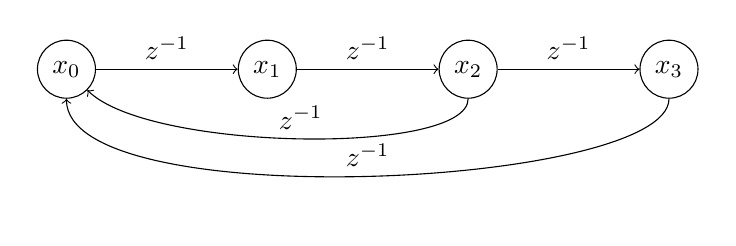
\begin{tikzpicture}
\matrix[ampersand replacement=\&,row sep=0.5cm, column sep=1.8cm]{
\node[draw,circle] (x0) {$x_0$}; \& \node [draw,circle](x1) {$x_1$}; \& \node [draw,circle](x2) {$x_2$};  \& \node[draw,circle](x3) {$x_3$}; \\ };
\draw[->] (x0) --node[above, midway]{$z^{-1}$}(x1);
\draw[->] (x1) --node[above, midway]{$z^{-1}$}(x2);
\draw[->] (x2) --node[above, midway]{$z^{-1}$}(x3);
\draw[->] (x2).. controls +(-90:1.1cm) and +(-45:1.1cm) ..  node[above, midway]{$z^{-1}$} (x0.south east);
\draw[->] (x3).. controls +(-90:1.5cm) and +(-90:1.5cm) ..  node[above, midway]{$z^{-1}$} (x0.south);
\end{tikzpicture}
\begin{eqnarray*}
x_0(k+1)&=& x_2(k)\oplus x_3(k) \\
x_1(k+1)&=& x_0(k) \\
x_2(k+1)&=& x_1(k) \\
x_3(k+1)&=& x_2(k)
\end{eqnarray*}
\end{frame}

\begin{frame}[containsverbatim]{M序列的产生方法及其性质}
取初始状态全为1,则各寄存器状态为
\begin{verbatim}
x0: 100010011010111
x1: 110001001101011
x2: 111000100110101
x3: 111100010011010
\end{verbatim}
%\begin{itemize}
%\item 1111(初态)→0111→0011→0001→1000 → 
%\item 0100 → 0010 → 1001 → 1100→ 
%\item 0110 →1011→0101→1010→1101→1110→1111
%\end{itemize}
输出序列为:111100010011010 (长度N=15)
\end{frame}

\begin{frame}{M序列的产生方法及其性质}
若寄存器个数为n,则有
\begin{itemize}
\item 周期长度$N=2^n-1$;
\item 总游程=$2^{n-1}$ ;
\item “0”出现次数为(N-1)/2,“1”出现次数为(N+1)/2.相差1次。
\end{itemize}
\end{frame}

\begin{frame}{二电平M序列及其性质}
\begin{itemize}
\item 将M序列转变成电平信号,
\begin{itemize}
\item “0”取为a,“1”取为-a。
\item 移位脉冲周期为$\Delta$,则该二电平M序列的周期为$N\Delta$。
\end{itemize}
\item 数字特征:
在一个周期$N\Delta$内,其均值$m_x$为 \\
\begin{eqnarray*}
m_x &=& \frac{1}{N\Delta}\left(\frac{N-1}{2}a\Delta-\frac{N+1}{2}a\Delta\right)=-\frac{a}{N} \\
\lim_{N\rightarrow \infty}m_x &=& 0
\end{eqnarray*}
\end{itemize}
\end{frame}


\begin{frame}{自相关函数$R_x(\tau)$}
$$
R_x{\tau}=\begin{cases}
\displaystyle \frac{-a^2}{N} & \scriptstyle (kN+1)\Delta<\tau<((k+1)N-1)\Delta  \\
\displaystyle a^2\left[ 1-\frac{(N+1)|\tau|}{N\Delta}\right] &\scriptstyle (kN-1)\Delta<\tau<(kN+1)\Delta
\end{cases}
$$
\end{frame}

\begin{frame}{三角脉冲分量与直流分量}
$$
R_x(\tau)=R^1_x(\tau)+R^2_x(\tau)
$$
其中:
\begin{description}
\item[$R_x^2(\tau)=\frac{-a^2}{N}$]为直流分量
\item[$R_x^1(\tau)=R_x(\tau)-R^2_x(\tau)$]为三角脉冲分量
\end{description}
\end{frame}

\begin{frame}
当$\Delta$很小时,$R_x^1(\tau)$可认为是脉冲函数,则有
\begin{eqnarray*}
R_x^1(\tau) &=& \frac{N+1}{N}a^2\Delta\delta(\tau) \\
R_x(\tau) &=& \frac{N+1}{N}a^2\Delta\delta(\tau)-\frac{a^2}{N}
\end{eqnarray*}
因此,M序列具有白噪声序列的数字特性。
\end{frame}

\section{M序列辨识系统的脉冲响应}

\begin{frame}{二电平M序列辨识系统的脉冲序列$g(\tau)$:作图法}
二电平M序列辨识$g(\tau)$有两种方法:作图法和公式法。首先介绍作图法:
\begin{eqnarray*}
R_{xy}(\tau) &=&  \int_{-\infty}^{\infty}g(\sigma)R_x(\tau-\sigma)d\sigma  \\
&=& \int_{0^+}^{N\Delta^-}g(\sigma)R_x(\tau-\sigma)d\sigma \\
&=& \int_{0^+}^{N\Delta^-}\left[\frac{N+1}{N}a^2\Delta\delta(\tau-\sigma)-\frac{a^2}{N}\right]g(\sigma)d\sigma \\
&=& \frac{N+1}{N}a^2\Delta g(\tau)-\int_{0^+}^{N\Delta^-}g(\sigma)d\sigma \\
&=& \frac{N+1}{N}a^2\Delta g(\tau)-A 
\end{eqnarray*}
其中:
$$
A=\int_{0^+}^{N\Delta^-}g(\sigma)d\sigma 
$$
\end{frame}

\begin{frame}
$R_{xy}(\tau)$可根据输入输出数据序列计算:
$$
R_{xy}(\tau)=\frac{1}{N}\sum_{i=1}^{N-1}x(i)y(i+\tau)
$$
只需将$R_{xy}(\tau)$曲线向上平移A,即可得$g(\tau)$。
%当$\tau\rightarrow \infty$时,$g(\tau)\rightarrow 0$.
\end{frame}

\begin{frame}{公式法求$g(\tau)$}
\begin{eqnarray*}
R_{xy}(\tau) &=& \frac{N+1}{N}a^2\Delta g(\tau)-\frac{a^2}{N}\int_0^{N\Delta}g(\sigma)d\sigma \\
\int_0^{N\Delta}R_{xy}(\tau)d\tau &=& \frac{N+1}{N}a^2\Delta \int_0^{N\Delta}g(\tau)d\tau \\
&& -\frac{a^2}{N}N\Delta\int_0^{N\Delta}g(\sigma)d\sigma \\
&=&\frac{\Delta a^2}{N}\int_0^{N\Delta}g(\tau)d\tau  \\
R_{xy}(\tau) &=& \frac{N+1}{N}a^2\Delta g(\tau)-\frac{1}{\Delta}\int_0^{N\Delta}R_{xy}(\sigma)d\sigma \\
g(\tau)&=&\frac{N}{(N+1)\Delta a^2}\left[R_{xy}(\tau)+\frac{1}{\Delta}\int_0^{N\Delta}R_{xy}(\sigma)d\sigma\right]
\end{eqnarray*}
\end{frame}

\begin{frame}{公式法求$g(\tau)$公式组}
\begin{eqnarray*}
g(\tau)&=&\frac{N}{(N+1)\Delta a^2}R_{xy}(\tau) +g_0\\
g_0 &=& \frac{N}{(N+1)\Delta^2 a^2}\int_0^{N\Delta}R_{xy}(\tau)d\tau \\
\int_0^{N\Delta}R_{xy}(\tau)d\tau &\approx & \Delta\sum_{i=0}^{N-1}R_{xy}(i) \\
R_{xy}(\tau) &=& \frac{1}{N}\sum_{i=0}^{N-1}x(i)y(i+\tau)
\end{eqnarray*}
\end{frame}

\begin{frame}{$g(\tau)$的矩阵表示}
离散维纳-霍夫方程:
\begin{eqnarray*}
R_{xy}(i\Delta) &=& \sum_{k=0}^{N-1}\Delta g(k\Delta)R(i\Delta-k\Delta) \\
R_{xy} &=& R g\Delta  \\
g&=& \frac{R^{-1} R_{xy}}{ \Delta }
\end{eqnarray*}
其中:
\begin{eqnarray*}
g &=& [g(0),g(1),\cdots,g(N-1)]^T \\
R_{xy} &=& [R_{xy}(0),R_{xy}(1),\cdots,R_{xy}(N-1)]^T \\
R &=&
\begin{bmatrix}
R_x(0) & R_x(-1)  & \cdots & R_x(-N+1)  \\
R_x(1) & R_x(0)   & \cdots & R_x(-N+2)  \\
\vdots & \vdots   &        & \vdots     \\
R_x(N-1) & R_x(N-2)   & \cdots & R_x(0)  
\end{bmatrix}
\end{eqnarray*}
\end{frame}

\begin{frame}{$g(\tau)$ 的矩阵表示:计 算$R^{-1}$ }
\begin{eqnarray*}
R_x(k) &=&
\begin{cases}
a^2 & k=0  \\
-\frac{a^2}{N}  & 1\leq k \leq N-1
\end{cases} \\
R &=& a^2
\begin{bmatrix}
1 & -\frac{1}{N} & \cdots & -\frac{1}{N}  \\
-\frac{1}{N} & 1 & \cdots & -\frac{1}{N}  \\
\vdots & \ddots  & \ddots & \vdots \\
-\frac{1}{N} & -\frac{1}{N} & \cdots & 1 
\end{bmatrix} \\
R^{-1} &=& \frac{N}{a^2(N+1)}
\begin{bmatrix}
2 & 1 & \cdots & 1 \\
1 & 2 & \cdots & 1 \\
\vdots & \vdots & \vdots & \vdots \\
1 & 1 & \cdots  & 2
\end{bmatrix}
\end{eqnarray*}
\end{frame}

\begin{frame}{$g(\tau)$的矩阵表示:计算$R_{xy}$}
\begin{eqnarray*}
R_{xy} &=& [R_{xy}(0),R_{xy}(1),\cdots,R_{xy}(N-1)]^T \\
&=&  \frac{1}{rN}XY \\
X&=&
\begin{bmatrix}
x(0) & x(1) & \cdots & x(rN-1) \\
x(-1) & x(0) & \cdots & x(rN-2) \\
\vdots & \vdots &  & \vdots \\
x(-N+1) & x(-N+2) & \cdots & x(rN-N) 
\end{bmatrix}\\
Y &=& \begin{bmatrix} y(0) & y(1) &\cdots & y(rN-1) \end{bmatrix}^T
\end{eqnarray*}
\end{frame}
\begin{frame}{$g(\tau)$的递推算法(在线辨识)}
递推算法:假设我们得到了$(m-1)$组观测数据时的辨识结果$g_{m-1}$,现在又得到了一组新的观测值$(x_m,y_m)$。现在讨论,就$g_{m-1}$与$(x_m,y_m)$数据来如何得到新的$g(\tau)$估计值$g_m$问题。

一般递推算法的计算公式形式如下:
$$
g_m = K g_{m-1} + \tilde{g}_m
$$
其中,$\tilde{g}_m$为从新得到的数据添加的信息。
\end{frame}

\begin{frame}{$R_{xy}$递推公式}
\begin{eqnarray*}
R_{xy}(i,m) &=& \frac{1}{m+1}\sum_{k=0}^m y(k)x(k-i) \\
&=& \frac{1}{m+1}\left[\sum_{k=0}^{m-1} y(k)x(k-i)+y(m)x(m-i)\right] \\
&=& \frac{1}{m+1}\left[mR_{xy}(i,m-1)+y(m)x(m-i)\right] \\
R_{xy}(m)&=& \frac{1}{m+1}\left[mR_{xy}(m-1)+y(m)X(m)\right] %\\
\end{eqnarray*}
其中:
\begin{eqnarray*}
R_{xy}(m) &=& [R_{xy}(0), R_{xy}(1), \cdots, R_{xy}(N-1)]^T \\
X(m) &=& [x(m),x(m-1),\cdots,x(m-N+1)]^T
\end{eqnarray*}
\end{frame}

\begin{frame}{$g(\tau)$递推公式}
\begin{eqnarray*}
g_m &=& \frac{R^{-1}R_{xy}(m)}{\Delta} \\
&=& \frac{R^{-1}}{\Delta}\frac{1}{m+1}\left[mR_{xy}(m-1)+y(m)X(m)\right] \\
&=& \frac{mR^{-1}R_{xy}(m-1)}{(m+1)\Delta}+\frac{R^{-1}}{(m+1)\Delta}y(m)X(m) \\
&=& \frac{m}{m+1}g_{m-1}+\frac{R^{-1}}{(m+1)\Delta}y(m)X(m) %\\
\end{eqnarray*}
\end{frame}

%    \begin{frame}{$g(\tau)$的矩阵表示}
%    在系统输入(r+1)个周期二电平M序列时,有
%    \begin{eqnarray*}
%    g &=& \frac{1}{a^2 r(N+1)\Delta}
%    \begin{bmatrix}
%    2 & 1 & \cdots & 1 \\
%    1 & 2 & \cdots & 1 \\
%    \vdots & \vdots & \vdots & \vdots \\
%    1 & 1 & \cdots  & 2
%    \end{bmatrix}
%    XY
%    \end{eqnarray*}
%    其中:
%    \begin{eqnarray*}
%    g &=&  \begin{bmatrix} g(0) & g(1) & \cdots & g(N-1) \end{bmatrix}^T  \\
%    X &=&  \begin{bmatrix}
%    x(0) & x(1) & \cdots & x(rN-1) \\
%    x(-1) & x(0) & \cdots & x(rN-2) \\
%    \vdots & \vdots & \vdots & \vdots \\
%    x(-N+1) & x(-N+2) & \cdots & x(rN-N) 
%    \end{bmatrix} \\
%    Y &=& \begin{bmatrix} y(0) & y(1) & \cdots & y(rN-1) \end{bmatrix}^T
%    \end{eqnarray*}
%    \end{frame}
%    
%    
%    \begin{frame}{$g(\tau)$的递推算法(在线辨识)}
%    递推算法:假设我们得到了$(m-1)$组观测数据时的辨识结果$g_{m-1}$,现在又得到了一组新的观测值$(x_m,y_m)$。现在讨论,就$g_{m-1}$与$(x_m,y_m)$数据来如何得到新的$g(\tau)$估计值$g_m$问题。
%    
%    一般递推算法的计算公式形式如下:
%    $$
%    g_m = K g_{m-1} + \tilde{g}_m
%    $$
%    其中,$\tilde{g}_m$为利用新观测值对g的预测值。
%    \end{frame}
%    
%    \begin{frame}{$R_{xy}$递推公式}
%    \begin{eqnarray*}
%    R_{xy}(i,m) &=& \frac{1}{m+1}\sum_{k=0}^m y(k)x(k-i) \\
%    &=& \frac{1}{m+1}\left[\sum_{k=0}^{m-1} y(k)x(k-i)+y(m)x(m-i)\right] \\
%    &=& \frac{1}{m+1}\left[mR_{xy}(i,m-1)+y(m)x(m-i)\right] \\
%    %&=& R_{xy}(i,m-1)+ \frac{1}{m+1}\left[-R_{xy}(i,m-1)+y(m)x(m-i)\right] 
%    R_{xy}(m)&=& \frac{1}{m+1}\left[mR_{xy}(m-1)+y(m)X(m)\right] %\\
%    \end{eqnarray*}
%    其中:
%    $$
%    X_m=[x(m),x(m-1),\cdots,x(m-N+1)]^T
%    $$
%    \end{frame}
%    
%    \begin{frame}{$g(\tau)$递推公式}
%    \begin{eqnarray*}
%    g_m &=& \frac{1}{rN\Delta}R^{-1}R_{xy}(m) \\
%    &=& \frac{R^{-1}}{rN\Delta}\frac{1}{m+1}\left[mR_{xy}(m-1)+y(m)X(m)\right] \\
%    &=& \frac{1}{m+1}\left[m\frac{R^{-1}}{rN\Delta}R_{xy}(m-1)+\frac{R^{-1}}{rN\Delta}y(m)X(m)\right] \\
%    &=& \frac{m}{m+1}g_{m-1}+\frac{R^{-1}}{(m+1)rN\Delta}y(m)X(m) %\\
%    % &=&  \frac{1}{rN\Delta} R^{-1} \{R_{xy}(m-1)\\
%    % && +\frac{1}{m+1}\left[-R_{xy}(m-1)+y(m)X_m\right]\} \\
%    % &=& g_{m-1}+  \frac{1}{m+1}\left[\frac{1}{rN\Delta}R^{-1}X_m y(m)-g_{m-1}\right] 
%    \end{eqnarray*}
%    \end{frame}

\section{脉冲响应序列求系统G(s)和G(z)}
\begin{frame}{脉冲响应序列求G(z)}
G(z)称为系统的脉冲传递函数,是系统的离散数学模型。
\begin{eqnarray*}
G(z)&=&\frac{C(z)}{R(z)}  \\
&=&\frac{b_0+b_1 z^{-1}+\cdots+b_n z^{-n}}{1+a_1 z^{-1}+\cdots+a_n z^{-n}}
\end{eqnarray*}
可得:
\begin{eqnarray*}
c_t+a_1 c_{t-1}+\cdots+ a_n c_{t-n} =  b_0 r_t+ \cdots + b_n r_{t-n}  \\
g(t)+a_1 g(t-1)+\cdots+ a_n g(t-n) =  b_0 \delta(t)+ \cdots + b_n \delta(t-n)
\end{eqnarray*}
\end{frame}
\begin{frame}
$$
\begin{bmatrix}
b_0 \\
b_1 \\
\vdots \\
b_0 
\end{bmatrix}
=
\begin{bmatrix}
1 & 0 & \cdots & 0 \\
a_1 & 1 & \cdots & 0 \\
\vdots & \ddots & \ddots & \vdots \\
a_n & a_{n-1} & \cdots & 1
\end{bmatrix}
\begin{bmatrix}
g(0) \\
g(1) \\
\vdots \\
g(n)
\end{bmatrix}
$$
$$
\begin{bmatrix}
g(1) & g(2) & \cdots & g(n)  \\
g(2) & g(3) & \cdots & g(n+1) \\
\vdots & \vdots &  & \vdots \\
g(n) & g(n+1) & \cdots & g(2n-1)
\end{bmatrix}
\begin{bmatrix}
a_n \\
a_{n-1} \\
\vdots \\
a_1
\end{bmatrix}
=
\begin{bmatrix}
-g(n+1) \\
-g(n+2) \\
\vdots  \\
-g(2n)
\end{bmatrix}
$$
\end{frame}

\begin{frame}{脉冲响应序列求G(s)}
G(s)称为系统的传递函数,是系统的连续数学模型。
$$
G(s)=\frac{C(s)}{R(s)}=\frac{M(s)}{N(s)}
$$

若系统具有n个两两互不相等的闭环极点$s_1,s_2,\cdots,s_n$.
则上式可分部因式为:
$$
G(s)=\frac{c_1}{s-s_1}+\frac{c_2}{s-s_2}+\cdots+\frac{c_n}{s-s_n}
$$
任务:已知$\{g(i)\}$及$n$,求$G(s)$中系数$c_i$和$s_i$.
\end{frame}

\begin{frame}{求$a_i$}
系统的脉冲传递函数为
$$
G(z)=\frac{b_0+b_1 z+ \cdots b_n z^n}{1+a_1 z + \cdots + a_n z^n}
$$
取$r(t)=\delta(t)$,则$c(t)=g(t)$。代入上式,写成差分方程为
$$
g(k)+a_1g(k+1)+\cdots+a_ng(k+n) = 0
$$
可得:
\begin{eqnarray*}
a_1g(k+1)+\cdots+a_ng(k+n) &=& -g(k) \\
\cdots &&  \\
a_1g(k+n)+\cdots+a_ng(k+2n-1) &=& -g(k+n-1)
\end{eqnarray*}
解上述$n$元一次方程组,可得$a_i$.
\end{frame}

\begin{frame}{求$s_i$}
由$G(s)$进行拉氏反变换可得:
$$
g(t)=c_1 e^{s_1 t} + c_2 e^{s_2 t} + ... + c_n e^{s_n t}
$$
所以:
\begin{eqnarray*}
g(t) &=& c_1 e^{s_1 (t)} + c_2 e^{s_2 (t)} + ... + c_n e^{s_n (t)}  \\
g(t+\Delta) &=& c_1 e^{s_1 (t+\Delta)} + c_2 e^{s_2 (t+\Delta)} + ... + c_n e^{s_n (t+\Delta)}  \\
\cdots && \cdots \\
g(t+n\Delta) &=& c_1 e^{s_1 (t+n\Delta)} + c_2 e^{s_2 (t+n\Delta)} + ... + c_n e^{s_n (t+n\Delta)}  \\
0 &=& c_1 e ^{s_1 t}[1+a_1 e^{s_1 \Delta} + \cdots + a_n e^{s_1 n\Delta}]  \\
&& +c_2 e ^{s_2 t}[1+a_1 e^{s_2 \Delta} + \cdots + a_n e^{s_2 n\Delta}] +\cdots  \\
&& +c_n e ^{s_n t}[1+a_1 e^{s_n \Delta} + \cdots + a_n e^{s_n n\Delta}] 
\end{eqnarray*}
可得$e^{s_i\Delta}$需满足的一元$n$次方程:
$$
1+a_1 e^{s_i \Delta} +a_2 [e^{s_i\Delta}]^2+\cdots+a_n[e^{s_i\Delta}]^n=0
$$
其中$i=1,2,\cdots,n$
\end{frame}

\begin{frame}{求$c_i$}
$$
g(t)=c_1 e^{s_1 t} + c_2 e^{s_2 t} + ... + c_n e^{s_n t}
$$
得:
\begin{eqnarray*}
g(0)&=& c_1 + c_2 + \cdots c_n \\
g(1)&=& c_1 e^{s_1 \Delta} + c_2 e^{s_2 \Delta}+\cdots+c_n e^{s_n \Delta} \\
&& \cdots \\
g(n-1)&=& c_1 e^{s_1 (n-1)\Delta} + c_2 e^{s_2 (n-1)\Delta}+\cdots+c_n e^{s_n (n-1)\Delta} \\
\end{eqnarray*}
\end{frame}

\begin{frame}{求解公式}
\begin{eqnarray*}
\begin{bmatrix}
g(k+1) & \cdots & g(k+n) \\
g(k+2) & \cdots & g(k+n+1) \\
\vdots & \vdots & \vdots \\
g(k+n) & \cdots & g(k+2n-1)
\end{bmatrix}
\begin{bmatrix}
a_1 \\ \vdots \\ a_n
\end{bmatrix}
&=&
\begin{bmatrix}
-g(k) \\ -g(k+1) \\  \vdots \\  -g(k+n-1)
\end{bmatrix} \\
1+a_1 x + \cdots a_n x^n &=& 0  \\
s_i&=&\frac{\ln x_i}{\Delta}  \\
\begin{bmatrix}
1 & 1 & \cdots & 1 \\
x_1 & x_2 & \cdots & x_n \\
\vdots & \vdots & \cdots & \vdots \\
x_1^{n-1} & x_2^{n-1} & \cdots & x_n^{n-1} \\
\end{bmatrix}
\begin{bmatrix}
c_1 \\ c_2 \\  \vdots \\ c_n
\end{bmatrix}
&=&
\begin{bmatrix}
g(0) \\ g(1) \\  \vdots \\  g(n-1)
\end{bmatrix}
\end{eqnarray*}

\end{frame}
% \section{思考}
% \begin{frame}{思考}
% \begin{itemize}
% \item 极大似然法辨识思想
% \end{itemize}
% \end{frame}


%\end{CJK*}
\end{document}
